\documentclass{article}
\usepackage[utf8]{inputenc}
\usepackage[UKenglish]{babel}
%\renewcommand{\familydefault}{\sfdefault}
\usepackage{ifpdf}
\usepackage{hyperref}
\usepackage{graphicx}
\usepackage{caption}
\usepackage{xspace}
\usepackage{comment}
\usepackage{xcolor,soul}

\usepackage{listings}
\usepackage{alltt}

\definecolor{light-gray}{gray}{0.850}

\newcommand{\hlc}[2][yellow]{\sethlcolor{#1}\hl{#2}}
\renewcommand{\c}[1]{\xspace{\small\hlc[light-gray]{\texttt{#1}}}\xspace}
\newcommand{\s}[1]{\xspace{\small\hlc[light-gray]{\textsl{#1}}}\xspace}

\renewcommand{\arraystretch}{1.5} % space between table rows

\lstset{ %
  backgroundcolor=\color{white},   % choose the background color; you must add \usepackage{color} or \usepackage{xcolor}
  basicstyle=\scriptsize,        % the size of the fonts that are used for the code
  breakatwhitespace=false,         % sets if automatic breaks should only happen at whitespace
  breaklines=true,                 % sets automatic line breaking
  captionpos=b,                    % sets the caption-position to bottom
  commentstyle=\color{mygreen},    % comment style
  deletekeywords={...},            % if you want to delete keywords from the given language
  escapeinside={\%*}{*)},          % if you want to add LaTeX within your code
  extendedchars=true,              % lets you use non-ASCII characters; for 8-bits encodings only, does not work with UTF-8
  frame=single,                    % adds a frame around the code
  keepspaces=true,                 % keeps spaces in text, useful for keeping indentation of code (possibly needs columns=flexible)
  keywordstyle=\color{blue},       % keyword style
  language=C,                 % the language of the code
  morekeywords={*,...},            % if you want to add more keywords to the set
  numbers=left,                    % where to put the line-numbers; possible values are (none, left, right)
  numbersep=5pt,                   % how far the line-numbers are from the code
  numberstyle=\tiny\color{gray}, % the style that is used for the line-numbers
  rulecolor=\color{black},         % if not set, the frame-color may be changed on line-breaks within not-black text (e.g. comments (green here))
  showspaces=false,                % show spaces everywhere adding particular underscores; it overrides 'showstringspaces'
  showstringspaces=false,          % underline spaces within strings only
  showtabs=false,                  % show tabs within strings adding particular underscores
  stepnumber=2,                    % the step between two line-numbers. If it's 1, each line will be numbered
  stringstyle=\color{black},     % string literal style
  tabsize=2,                       % sets default tabsize to 2 spaces
  title=\lstname                   % show the filename of files included with \lstinputlisting; also try caption instead of title
}

\title{Ceph Mon: a technical overview}
\author{Paolo VIOTTI}
\date{\today}
\ifpdf
\hypersetup{
    pdfauthor={Paolo VIOTTI},
    pdftitle={Ceph Mon: a technical overview},
}
\fi
\begin{document}

\maketitle

\begin{abstract}
Ceph is a free software storage platform designed to provide object, block and file storage 
using computer clusters running on commodity hardware. 
Ceph's main design goals include high scalability, fault tolerance and low maintenance requirements.
This document provides an in-depth technical overview of the design of Ceph Monitor, 
i.e. the Ceph component in charge of maintaining a map of the cluster along with authorization information.
\end{abstract}

\section{Ceph: an introduction}
Ceph \cite{ceph} is a free software storage platform that provides object, block and file storage 
using computer clusters running on commodity hardware. 
Since its origin as a research project around 2006, 
Ceph has undergone constant and substantial development,
thus gaining popularity which is reflected by an ever increasing adoption as storage backend in state-of-the-art
high-end computing systems \cite{ceph-openstack}.

As illustrated in Fig. \ref{fig:stack}, Ceph exposes to application clients multiple APIs: 
\begin{itemize}
	\item a POSIX-compatible distributed file system (\textbf{Ceph FS}), built as Linux kernel module or user-space FUSE client;
	\item a REST-based storage gateway (\textbf{RADOSGW}) compatible with OpenStack Swift and Amazon S3;
	\item a block storage device (\textbf{RDB}) suitable for virtualization platforms making use of kernel 
	virtualization technologies such as QEMU or KVM.
\end{itemize}

\begin{center}
	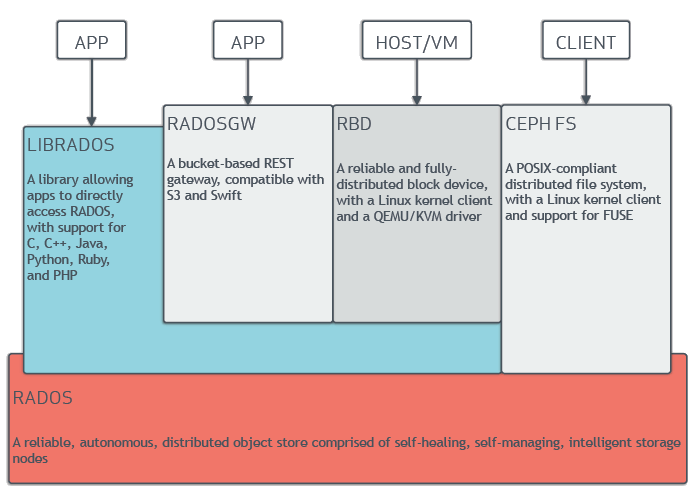
\includegraphics[scale=0.35]{figs/ceph-stack.png}
	\captionof{figure}{Ceph application stack (courtesy of ceph.com)}
	\label{fig:stack}
\end{center}

Beside, an application developer may even hook into the low level API exposed through \textbf{librados} 
and offered in several programming languages in order to directly connect with \textbf{RADOS} 
(\textit{Reliable Autonomic Distributed Object Store}), i.e. the inner object storage layer
that acts as foundation of the interfaces mentioned above.

The Ceph cluster consists of different components, running as distributed daemons:
\begin{itemize}
	\item Cluster monitors (\textit{ceph-mon}, or Mon) that keep track of active and failed cluster nodes;
	\item Metadata servers (\textit{ceph-mds}) that store the metadata of inodes and directories;
    \item Object storage devices (\textit{ceph-osd}) that actually store data on local filesystems;
    \item RESTful gateways (\textit{ceph-rgw}) that expose the object storage layer as an interface 
    compatible with Amazon S3 or OpenStack Swift APIs.
\end{itemize}

The rest of this document focuses on the monitor component, starting from its high-level architecture,
deep down to the implementation details present, to date, in its C++ codebase \cite{ceph-code}.
To marry the need for this 1000 ft. view with the requirement of presenting the related 
low level features, in the following sections informal functional descriptions may be presented beside
the name of their main corresponding entities in the code (e.g. \c{classes} or \s{data structures}).
Most of the code required to run the monitor is contained in the \texttt{src/mon} directory of the repository  \cite{ceph-code}
($\sim$34k LOC), although it shares with the rest of the codebase few functions and classes related to
specific parts of the system (e.g. OSD or MDS daemons, respectively in \texttt{src/osd} and \texttt{src/mds}),
or networking, logging and other basic facilities.

\section{Ceph Mon}
A Ceph Monitor maintains a set of structured information about the cluster state, including:

\begin{itemize}
	\item the monitor map - \c{MonMap}
	\item the OSD map - \c{OSDMap}
	\item the Placement Group (PG) map - \c{PGMap}
	\item the MDS map - \c{MDSMap}.
\end{itemize}

Additionally, information about authorization and capabilities granted to users over the 
different components of the system is maintained. 
Besides, Ceph holds a history, as a sequence of \textit{epochs}, of each state change in the maps.
All these information are replicated across the ceph-mon instances - 
which are, for example, 3 or 5, deployed on different machines.
Each monitor replica keeps its data strongly consistent using an implementation of the 
Paxos consensus algorithm (\c{Paxos}).

\subsection{Architecture}

As illustrated in Fig. \ref{fig:monarch}, the Ceph monitor is composed by several sub-monitors which 
oversee different aspects of the cluster.
All these monitors refer to a unique instance of Paxos\footnote{This was not true before v0.58,
see: \url{http://ceph.com/dev-notes/cephs-new-monitor-changes/}}
in order to establish a total order between possibly concurrent operations and achieve strong consistency.
The Paxos instance is agnostic of any semantic associated with the updates it helps ordering, as in fact
it just delivers blobs (i.e. \s{bufferlist} as payload of \c{Message}).

\begin{center}
	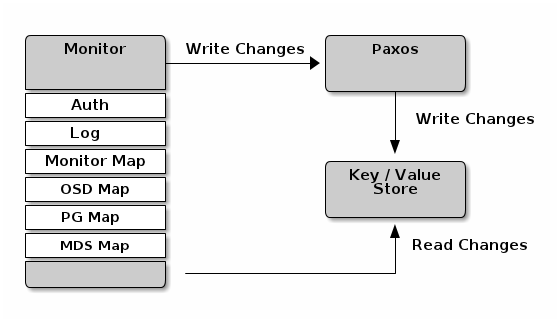
\includegraphics[scale=0.50]{figs/ceph-mon-arch.png}
	\captionof{figure}{Ceph Monitor high-level architecture (courtesy of ceph.com)}
	\label{fig:monarch}
\end{center}

\subsection{Implementation details}

As depicted in Figure \ref{fig:monclass}, the \c{Monitor} object acts as container and coordinator of different objects.

\begin{center}
	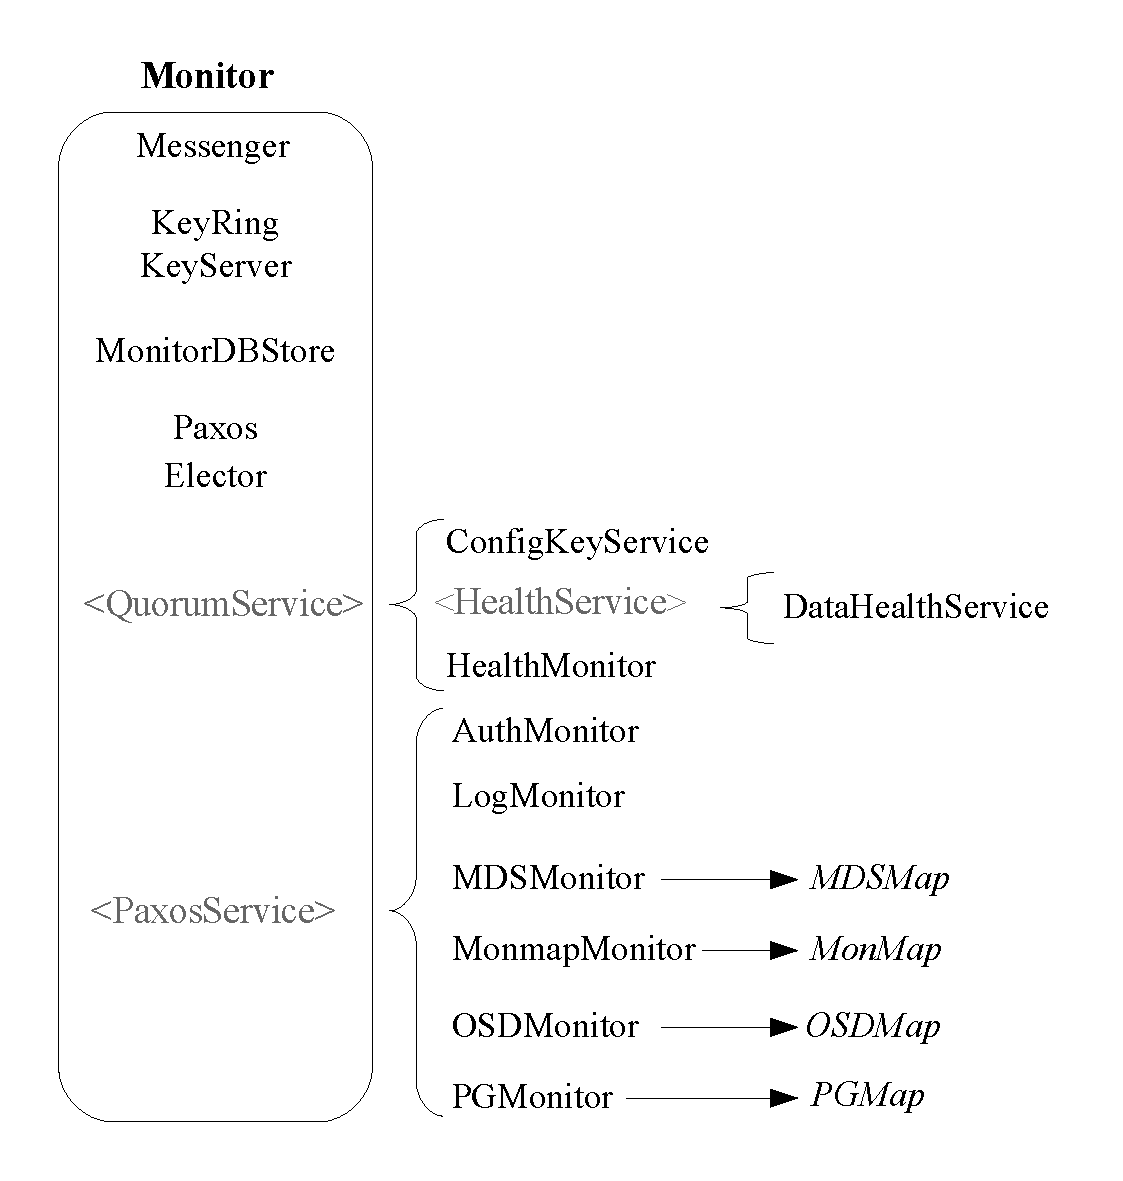
\includegraphics[scale=0.50]{figs/class_dia.pdf}
	\captionof{figure}{Ceph Monitor classes}
	\label{fig:monclass}
\end{center}

Some of them inherit from a common parent class named \c{QuorumService}.
In particular, \c{HealthMonitor} holds a reference to \c{DataHealthService}, 
which is in turn child class of \c{HealthService}.
\c{DataHealthService} is responsible of periodically sharing with other quorum members
or presenting to the admin user some statistics about general cluster health.
\c{KeyConfigService} is another subclass of \c{QuorumService} which uses \c{Paxos}
in order to propagate to the monitor cluster members 
the addition or removal of cryptographic material to the local store.

\paragraph*{}
Beside the above mentioned classes, other singleton objects take part in the
general functioning of the monitor as explained in the following list.

\begin{itemize}
	\item[\c{Messenger}] in charge of the network communications with other parties;
	\item[\c{KeyRing} and \c{KeyServer}] manage keying material for authorization;
	\item[\c{MonitorDBStore}] manages the local database (i.e. LevelDB) which stores maps and cryptographic material;
	\item[\c{Paxos}] Paxos implementation;
	\item[\c{Elector}] used only to maintain the local state during elections.
\end{itemize}

Finally, few classes which inherit from \c{PaxosService} are properly named \c{*Monitor} as they
implement the logic to maintain the maps of the different sections of the Ceph cluster.
Aside from \c{AuthMonitor}, which is responsible for enabling or disabling capabilities on a user basis,
and \c{LogMonitor}, which tunes logging as required by the administrative user,
all other \c{*Monitor}s refer to specific classes named \c{*Map} to save their pertaining states.
Such maps are also serialized to the local key-value store (i.e. LevelDB)
which is managed by \c{MonitorDBStore}.
To guarantee total ordering of updates, every change on maps is submitted to the Paxos service
and then applied only once the related Paxos proposal has been committed.

\begin{comment}
Table \ref{tab:class} shows an incomplete list of classes involved in the functioning of the monitor.
To each class is
\begin{center}
	\begin{tabular}{l|p{6cm}|p{5cm}}
		Entity & Purpose & Data and attributes \\ \hline
		\texttt{ceph\_mon.cc} & main entry point for monitor daemon and batch commands & - \\
		\c{Monitor} & 
		
		the main Monitor class 
		\begin{itemize}
		\item holds and start \c{Paxos}, 
		                 \c{MonitorDB}, \c{Messenger} and all the sub-monitors
		                 (\c{*Monitor}) 
        \item dispatch messages coming from \c{Messenger} to the sub-monitors 
        \end{itemize}		                 
		                 
		                 & 
		                \c{MonMap}, \c{KeyServer}, \c{KeyRing}, \c{Paxos},
		                \c{MonitorDBStore}, \c{*Monitor}\\
		%${41} & ${42} & ${43} \\\\
	%${101} & ${102} & ${103} \\\\
	\end{tabular}
	\captionof{table}{Main classes used by Ceph Monitor}
	\label{tab:class}
\end{center}
\end{comment}

%During runtime operations, Ceph OSD Daemons check up on other Ceph OSD Daemons and report their findings to the Ceph Monitor.

The monitor can assume the following states during an execution:
\begin{itemize} \itemsep1pt
\item \textit{probing}: initial and bootstrap phase state;
\item \textit{synchronizing}: used when synchronizing the state due to significant drifting from leader's replica;
\item \textit{electing}: assumed when starting or joining a Paxos election;
\item \textit{leader}: the monitor is active and leader in the Paxos quorum; 
\item \textit{peon}: the monitor is active and follower in the Paxos quorum;
\item \textit{shutdown}: when shutdown process is ongoing.
\end{itemize}


\subsection{Paxos}
The \c{Paxos} class implements the Paxos algorithm in order to guarantee agreement over the ordering of changes performed 
on Ceph maps.
Apart from a couple of online informal or incomplete documents \cite{ceph-paxos1,ceph-paxos2}, 
the only reliable source of documentation available about this Paxos implementation is contained
in the comments of the Paxos class and header files.
In particular, there is included the following excerpt, which reports about the difference between the Paxos algorithms
and this practical implementation.

\begin{alltt}
\small
This libary is based on the Paxos algorithm, but varies in a few key ways:
 1- Only a single new value is generated at a time, 
    simplifying the recovery logic.
 2- Nodes track "committed" values, 
    {\em and share them generously (and trustingly)}
 3- A 'leasing' mechanism is built-in, allowing nodes to determine 
    when it is safe to "read" their copy of the last committed value.
\end{alltt}

Paxos tracks the last and the first committed key number on the store, along with each numbered key and their 
corresponding values that have been committed thus far.
As mentioned before, values are binary blocks opaque to Paxos.
A trimming mechanism guarantees that the number of Paxos states kept in the local databases is limited
according to a configuration paramenter.


The state diagram shown in Figure XXX presents the states Ceph's Paxos can assume and their transitions.





\subsection{Additional notes}

\begin{verbatim}
To ask / understand:
 
 - MonitorStore.{h,cc} never used: obsolete?
 - difference between MonCommands and DumplingMonCommands?
 - functional difference between QuorumService and PaxosService 
    (since they both contain refererences to Paxos and the Monitor)?
\end{verbatim}


\begin{thebibliography}{1}

  \bibitem{ceph} Ceph storage platform. \url{http://ceph.com/} 

  \bibitem{ceph-openstack} OpenStack User Survey Insights: November 2014. \\
  \url{http://perma.cc/367D-G5YN} 
  
  \bibitem{ceph-code} Ceph source code. \url{https://github.com/ceph/ceph} 
  
  \bibitem{ceph-paxos1} Ceph's new monitor changes. \url{http://ceph.com/dev-notes/cephs-new-monitor-changes/} March 7th, 2013
  
  \bibitem{ceph-paxos2} Monitors and Paxos, a chat with Joao. \url{http://ceph.com/community/monitors-and-paxos-a-chat-with-joao/} September 10th, 2013

  %\bibitem{fo} Bob Tadashi Wakabayashi {\em Anti-Foreignism and Western
  %Learning in Early-Modern Japan} 1986: Harvard University Press.

\end{thebibliography}
	
\end{document}
